\documentclass[a4paper,11pt,twoside]{report}%pridat twoside, do [] pre obojstrannu tlac
    \pagestyle{headings}
    \usepackage[top=2.5cm, bottom=2.5cm, left=3.5cm, right=2cm]{geometry} %odporucane okraje

\usepackage[utf8x]{inputenc}
\usepackage[T1]{fontenc} %pekne makcene
\usepackage{algorithmic}
\usepackage{algorithm}
\usepackage{amsmath}
\usepackage{amssymb}
\usepackage{graphicx}
\usepackage{graphics}
\usepackage{cite}

\graphicspath{ {pictures/} }
\renewcommand{\thesection}{\arabic{section}}

\author{Matus Behun}
\title{Cayley graphs of given diameter on linear groups}

\usepackage{hyperref}
    \hypersetup{colorlinks,citecolor=red,filecolor=black,linkcolor=blue,urlcolor=blue,pdftex}

\begin{document}
\setlength{\belowdisplayskip}{7pt} \setlength{\belowdisplayshortskip}{5pt}
\setlength{\abovedisplayskip}{7pt} \setlength{\abovedisplayshortskip}{5pt}

%====================================================================================================================================================
% FIRST PAGE 
%====================================================================================================================================================
\thispagestyle{empty}
{
	\topmargin=0pt
	\centerline {\large \bf{SLOVAK UNIVERSITY OF TECHNOLOGY}}
	\vskip 0.2cm
	\centerline{\large \bf{FACULTY OF CIVIL ENGINEERING}}
	\vskip 5cm
	\centerline{\Large \bf{Cayley's graph of given diameter on linear groups}}
	\vskip 0.2cm
	%\centerline{\Large \bf{HÝ JEHO DRUHÝ RIADOK}}
	%\centerline{ \bf{(verzia z~\today) }}   %vypisovanie dnesneho datumu
	\vskip 0.5cm
	\centerline{\large \bf{Bachelor's thesis}}
	\vskip 5cm          %\vskip 2cm             %zmena kvoli zobrazovaniu dnesneho datumu
	\normalsize
		\begin{tabular}[l]{p{0.27\textwidth}p{0.73\textwidth}}
		Študijny program: & Matematicko-počítačové modelovanie\\
		Študijny odbor: & Aplikovaná matematika\\
		Školiace pracovisko: & doplň ma\\
		Vedúci diplomovej práce: & doplň ma \\
		\end{tabular}
	\vskip 3cm
	\centerline{\large \bf{BRATISLAVA 2018}}
	\vskip 0.2cm
	\centerline{\large \bf{Matúš Behun}}
}

\pagebreak
\tableofcontents
\newpage
%====================================================================================================================================================
% END OF FIRST PAGE  
%====================================================================================================================================================

\section{Introduction}


%====================================================================================================================================================
% INTRODUCTION TO DEGREE DIAMETER PROBLEM ON UNDIRECTED GRAPHS strana 8, 9
%====================================================================================================================================================

%%% Pridat ako sa modeluju grafy podla prednasky? %% Opytat sa
%%% Pridat o akych grafoch uvazujeme len pre SVOC %% Opytat sa

\section{Degree/diameter problem}
\subsection{Moore's boundary}
%% Uvod do problemu 
Degree/Diameter problem's concerning construction of graphs with biggest possible order $n_{d,k}$ with given diameter $k$ and maximal degree $d$. There exists theoretical upper boundary named after Moore for such graphs. 

Boundary is easily derived from construction of graph with node connected to $d$ nodes. Next step consists of making every of new $d$ nodes making adjacent to $d-1$ nodes making them of degree $d$. There have to $n$ such steps including step for first one to satisfy diameter restriction.

\begin{equation}
	\begin{split}
		n_{d,k} \leq M_{d,k}	& = 1 + d + d(d - 1) + \dots + d(d - 1)^{k-1}  \\
				 				& = 1 + d(1 + (d - 1) + \dots + (d - 1)^{k-1}) \\
				 				& =	\begin{cases}
										1+d\frac{(d-1)^{k}-1}{d-2}, & \text{if}\ d > 2 \\
										2k+1, & \text{if}\ d=2 
									\end{cases}
	\end{split}
\end{equation}

%% About upper boundary
\subsection{Moore's graphs}
	 Graphs which's order is equal to Moore's boundary are called Moore's graphs. 
Such graph is necessary regular of degree $d$. Research of Moore's graph was initiated by Hoffman and Singleton in paper with focus on diameter 2 and 3. ~\cite{Hoffman-Singleton}
They proved there are Moore's graphs for $k=2, d=2,3,7$ wich are unique and possibly $57$ which hasn't been found yet. They also proved that heptagon is unique Moore's graph of degree 3 and diameter 2. 

The proofs exploit eigenvalues and eigenvectors of the adjacency matrix (and its principal submatrices) of graphs. \\ \\
Let A be the adjacency matrix of a graph of degree d $\geq$ 2, k = 2 and order
\begin{align*}
	n = M_{d,2} = 1 + d + d(d - 1) = d^2 + 1
\end{align*}
Diameter 2 of graph makes matrix A satisfy equation with I being identity and J being all-ones matrix.
\begin{equation*}
	A^2 + A - (d - 1)I = J
\end{equation*}
Since eigenvalues of A and J must satisfy the same polynomial equation and the spectrum of J is $n^{1}0^{n-1}$, it follows that A has just two eigenvalues r, s distinct from d and these satisfy the equation
\begin{equation*}
	x^2 + x - (d - 1) = 0 
\end{equation*}
that is 
\begin{equation*}
	r,s = (-1 \pm \sqrt{4d - 3})/2  
\end{equation*}
For multiplicities a,b of r,s one obiously has a+b= $d^2$ and the trace of A gives  

\begin{equation*}
	trace(A) = 1 \ast d + a \ast r + b \ast s = 0 
\end{equation*}
If r and s are irrational, then a = b and d = 2. If r,s are rational, then they must be integral; also, then 4d - 3 = $m^{2}$, for some positive integer m. Letting b = $d^{2}$ - a and then substituting d = ($m^2$ + 3)/4 into the trace equation yields, after simplification, a polynomial equation for m of the fifth degree (with parameter a) with leading coefficient 1 and absolute term equal to 15. Then m must be a divisor of 15 and hence m $\in$ \{1,3,5,15\}, that is, d $\in$ \{1, 3, 7, 57\}.
$\blacksquare$

Easily found Moore graphs for parameters $d=2$ and k $\geq$ 2 are circle graphs $C_{2k+1}$, Moore graphs with diameter k=1 and degree d $\geq$ 1 are complete graphs $K_{d+1}$. Unique Moore's graph for $n_{3,2}$ is Petersen graph and for $n_{7,2}$ Hoffman-Singleton graph.

\begin{figure}[!ht]
	\centering
	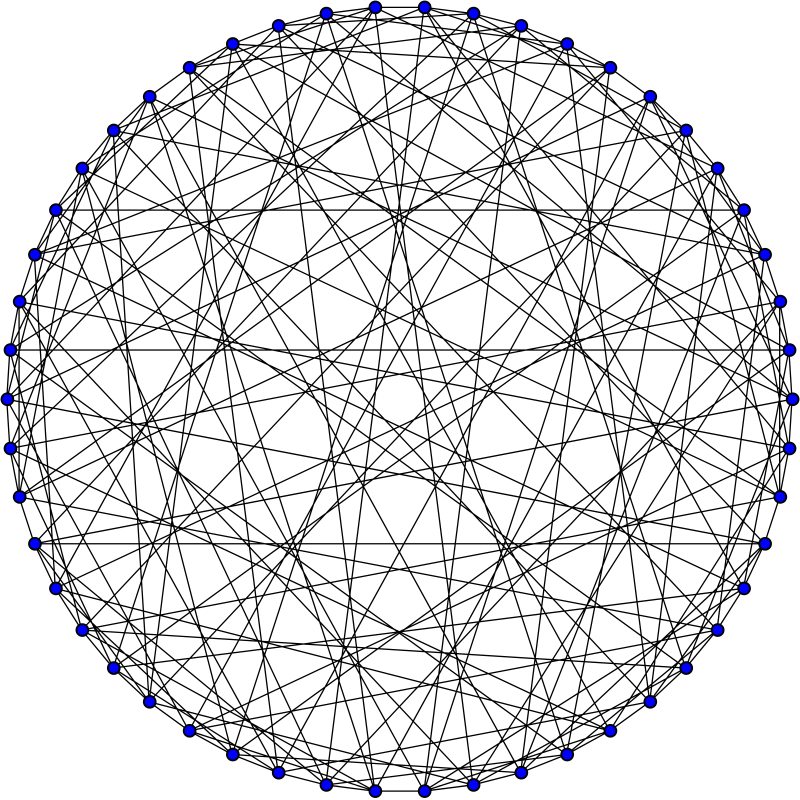
\includegraphics[scale=0.33]{Hoffman-Singleton_graph.png}
	\caption{Hoffman-singleton graph is Moore's graph with $d=7$ and $k=2$ }
\end{figure}

%====================================================================================================================================================
% END OF INTRODUCTION TO DEGREE DIAMETER PROBLEM
%====================================================================================================================================================

%====================================================================================================================================================
% GRAPHS NON MOORE'S  
%====================================================================================================================================================

\subsection{Graphs close to Moore boundary}
Because there are only few graphs mentiond earlier that satisfy theoretical Moore's boundary there has been effort making graphs as close as possible. Graph with defect is denoted by (d,k,$-\delta$) equal to graph of order $M_{d,k}-\delta$. Conventionally $\delta$ refers to small defect $\delta$ $\leq$ d. 

Research yields many results concerning graph with defects. Erdős, Fajtlowitcz and Hoffman proved~\cite{Erdos-Fajtlowicz-Hoffman} that there is no graph of degree d and diameter 2 and $\delta$ = 1 apart from cycle $C_{4}$.  
Concerning $\delta = 2$ in case of $d = 2 (d,k,-2)$ graphs are cycles $C_{2k-1}$. For $d \geq 3$, only five graphs are known at present two $(3,2,-2)$ of order 8, $(4,2,-2)$ of order 15, a $(5,2,-2)$ of order 24 and $(3,3,-2)$ of order 20.

%% Doplnit citacie
\subsection{Constructions of large graphs}
Different aproach to finding graphs close to Moore bound is by constructing large graphs to find lower bound on the maximum possible order of graphs. There were various ways to consider these techniques such as vertex-transitive and Cayley graphs. For finding such graphs there are many techniques have been used such as star product, the voltage assignment technique, graph compounding and computer search. \\

\subsection{Cayley graph definition}
Let $\Gamma$ be a group and let S be a symmetric S = $S^{-1}$ generating set without identity element  $e\not\in$ S. The $\textit{Cayley graph}$ $C(\Gamma,S)$ is the graph with vertex set $\Gamma$, with vertices a,b being adjacent if $a^{-1}b$ $\in$ S.

Let Cayley graph graphs with degree d and diameter k denote by $C_{d,k}$. Proved in ~\cite{Jajcay-Macaj-Siran} there exists $d \geq 3$ and $c \geq 2$ there exists a set S of natural numbers of positive density s.t. $C_{d,k} \leq M_{d,k}-c$ for all D $\in$ S. There is no better upper bound on $C_{d,k}$ than $M_{d,k} - 2$. For other pairs there is no upper bound on $C_{d,k}$ than $M_{d,k} - 2$.
 
Best available lower bound on $C_{d,2}$ was obtained by Šiagiová and Širáň. Let $D = \{ 2^{2m+\mu}+(2+\delta)2^{m+1}-6,m \geq 1, \mu \in \{0,1\} \}$ and $d$ be from set D then bound is $C_{d,k} > d^{2} - 6\sqrt{2}d^{3/2}$.

\subsection{Graph lifting}
Graph lifting is technique producing large graphs and is well known in topological and algebraic graph theory.~\cite{Gross-Tucker} 

%% Correct definition from papers
Description of $\textit{voltage assignment}$ assume that graph is unoriented and orientation is chosen but fixed for every edge and we assign each of them element of group. Formally: 

Let $\Gamma$ be a finite group, map:
\begin{align*}
	\alpha: E(G) \rightarrow \Gamma
\end{align*}	
will be called voltage assignment if $\alpha(e^{-1})$ = $(\alpha(e))^{-1}$, for any edge $e \in E(G)$. Bigger graph $G^{\alpha}$ is called lift while:  
\begin{align*}
	V(G^{\alpha}) = V(G) \times \Gamma \\
	E(G^{\alpha}) = E(G) \times \Gamma 
\end{align*}	

%% Example of Hoffman-Singleton lift.

Bigger graph $G$ is a lift if and only if the automorphism group of $G$ contains a non-trivial subgroup acting freely on the vertex set of $G$.~\cite{Gross-Tucker} Many current biggest $n_{d,k}$ graphs can be described as lifts. For example $n_{3,7}$, $n_{3,8}$, $n_{4,4}$, $n_{5,3}$, $n_{5,5}$, $n_{6,3}$, $n_{6,4}$, $n_{7,3}$, $n_{14, 3}$ and $n_{16,2}$ were obatained by computer search.~\cite{Exoo} Lifting of graph consiting of one vertex with are Cayley graphs. 

\subsection{Table of large graphs}
\subsection{Table of large Cayley's graphs}

\bibliography{degree-diameter}{}
\bibliographystyle{plain}
\end{document}
